\documentclass[review]{elsarticle}

\usepackage{booktabs} % For formal tables

\usepackage{lineno,hyperref}

\modulolinenumbers[5]

\journal{Journal of \LaTeX\ Templates}

%% `Elsevier LaTeX' style
\bibliographystyle{elsarticle-num}
%%%%%%%%%%%%%%%%%%%%%%%

\begin{document}

\begin{frontmatter}

\title{Distributed Task Execution: Designing A Flexible Framework For Managing Distributed Workloads in Apache Airavata}

%% Group authors per affiliation:
\author{Gourav Shenoy}
\author{Ajinkya Dhamnaskar}
\author{Suresh Marru}
\author{Marlon Piece}

\address{Science Gateways Research Center, Pervasive Technology Institute}
\address{Indiana University, Bloomington, IN 47408, USA}

\begin{abstract}
Managing workloads for both compute-intensive and data-intensive applications is a fundamental task for science gateways in order to provide resilient, scalable and manageable infrastructure. Scientific applications by nature are mostly compute-expensive and require high-end computational resources and may require long execution times. Based on the problems, some executions may either require or result in large datasets. Technology evolutions (occasionally disruptive) challenge the scientific application execution frameworks to adapt to paradigm changes. Cloud Computing has added on demand computing to the traditional batch queue based computing. In this paper we discuss a system design which divides workload management logic into distributed components. This design is inspired by microservice architectural principles to exploit their potential for scalability, availability, portability and, most importantly, ability to support rapid evolution. We encapsulate diverse execution patterns as Directed Acyclic Graph (DAG), thus alleviating the framework from computational paradigm changes. By capturing execution patterns as a graph, the framework itself can be generic, and the differences are encapsulated into the DAG descriptions. The DAG enactment is achieved by loosely-coupled components with well-defined communication contracts. We discuss the motivations for such a design and early validations with Apache Airavata as an implementation laboratory. 
\end{abstract}

\begin{keyword}
Apache Airavata, Science Gateways, Distributed Systems
\end{keyword}

\end{frontmatter}

\linenumbers

\section{Introduction}

Cyberinfrastructure is the collection of distributed computing resources, research networks, and software. Central problems in cyberinfrastructure operations involve adapting and bridging patterns \cite{hey2005cyberinfrastructure}. Cyberinfrastructure must adapt to both the resource-centric views that are typically adopted by computing resource providers and the scientific or application-centric views of cyberinfrastructure of end users. Cyberinfrastructure must also bridge between multiple infrastructure providers. Science gateway research addresses both problems by providing web-based user interfaces and middleware services to support scientific users and communities. Science gateways by their nature provide user-centric views of infrastructure, focusing on scientific applications used by a specific field (atmospheric science, bio-informatics, computational chemistry, nanotechnology, phylogenetics, etc). Gateways also frequently need to provide access to multiple grids, local campus resources, and computing clouds to serve their communities \cite{perera2008workflow}. Gateways thus act as overlay cyberinfrastructure, federating resources that do not otherwise interoperate. Science gateway research looks for ways to encapsulate these problems within a single software framework. In this paper, we examine these requirements in greater detail, propose an architectural solution, and investigate the implementation of this solution within the Apache Airavata framework \cite{marru2011apache,marru2015apache}. 

Two fundamental considerations in designing science gateway architectures is that they are deployed to support distributed systems and that they are distributed systems in their own right.   A distributed system is an application that executes a collection of protocols to coordinate the actions of multiple processes on a network, such that all components cooperate together to perform a single or small set of related tasks. The fundamental benefit of such a system is the ability to connect remote users with remote resources in an open and scalable fashion. When we say open, we mean each component is continually open to interaction with other components. When we say scalable, we mean the system can easily be expanded to accommodate changes in the number of users, resources and computing entities.  Therefore, a fundamental goal in designing a gateway architecture is to not compromise system reliability.  Airavata is a stable and reliable gateway middleware, which was a difficult goal to achieve, given the complexity of interactions between different distributed components which are running simultaneously \cite{pierce2015apache}. Our proposed design for gateway architecture is able to enhance gateway flexibility without compromising reliability.

In order to achieve reliability, a distributed system needs to be fault-tolerant, highly-available, consistent, scalable, secure, and responsible \cite{burns2016design, casavant1988taxonomy}. Each of these characteristics has its own set of design challenges, and designing architectures and applications in distributed environments adds a layer of complexity to those challenges.  Below we discuss several factors that need to be considered when designing any distributed application.

\textbf{Abstraction}: Simplicity is a key ingredient for the success of any computing application; most users do not care about lower-level infrastructure details. Typically users are interested in an application's responsiveness, availability and correctness. A major challenge for any distributed system is the ability to scale dynamically, without burdening the user or compromising the usability. 

\textbf{Disruptive technologies and the opportunities}: Emerging needs and competing markets strive to come up with disruptive solutions to distributed environment problems. Technologies like HTCondor \cite{tannenbaum2001condor,thain2005distributed}, actor-based models such as AKKA \cite{akka}, Spark \cite{zaharia2010spark}, and others have examined the problems of distributed workload management. Our solution to the problem is an amalgamation of the design inspirations from these technologies. Design decisions are heavily influenced by the nature of an application. Distributed applications are broadly classified as data-intensive and compute-intensive. Data-intensive applications devote most of their time processing large amounts of data (typically terabytes or petabytes) and processing I/O. On the other hand, compute-intensive applications demand a lot of computing power. Most of the scientific applications are compute-intensive and require supercomputers to execute jobs. Many scientific applications are hard to execute on local workstations because of their high-end resource requirements. These applications run best on supercomputers or clouds.

\textbf{Heterogeneity of compute resources}: A core responsibility of science gateways is to provide simplified access to diverse computing resources.  By definition, heterogeneous computing resources are hard to generalize and can be designed and configured based on usage needs. HPC (High Performance Computing) and HTC (High Throughput Computing) are heavily practiced computing paradigms, and each is uniquely suited for particular types of computing problems. HPC is tailored to large computational tasks that require interactions of intermediate results to complete the computation.  HPC focuses on executing jobs that require large computing power for short duration. HTC, on the other hand, is suited to problems with large computational loads where individual computations do not need to interact while running.   HPC can be roughly termed as parallel computing on high end computing resources, and this environment is best suitable for Message Passing Interface (MPI) workloads which demand low latency and where tasks are tightly-coupled.  Similarly, we also note the growing importance of data-centric computing and real-time computing. While HPC and HTC still dominate traditional scientific computing, new communities of users and new opportunities exist if gateways can flexibly accommodate these computing usage patterns. 

In summary the diversity of these parallelism patterns is exemplified by the diversity in programmed languages and their associated run time systems. These patterns  vary from simple single-threaded to multi-threaded and parallel implementations. This diversity motivates our problem to explore an architecture pattern which is easy to implement and yet facilitates evolution. 

\section{PROBLEM STATEMENT}

\subsection{Apache Airavata and Distributed Components}
Apache Airavata is open source science gateway middleware that has been described previously in \cite{pierce2014apache}\cite{marru2015apache}. Airavata is used to power production science gateways, but we also use it as a laboratory to explore cyberinfrastructure research and distributed computing problems, such as the work described here.

Apache Airavata is designed to act as a multi-tenanted platform that can be used by multiple gateways simultaneously through a secure, well-defined API and data models that are defined using Apache Thrift.   In Airavata's abstract architecture, we identify the following major components: a) the API server, which is the interface between Airavata and client gateways; b) the Registry, which serves as the repository for system metadata; c) the Task Executor (sometimes called GFAC), which manages the lifecycle of task executions on remote resources; and d) the Orchestrator, which converts abstract task execution requests into concrete requests and routes them to the specific Task Executors that can fulfill request.  Airavata uses third party services for managing user identity and securing client gateway-API Server connections.  

Components in Airavata may communicate by both messaging and direct RPC calls.  The Thrift-defined API includes data models that can be exchanged between components as well as between the gateway and the API server.  We have found in practice that hybrid notification-RPC communications work well: a component may be notified via the message bus to contact another component by direct call.

In this paper, we focus on the interactions between the Orchestrator and the Task Executor components, reimplementing both components from scratch and rethinking their roles in the abstract architecture. We are particularly interested in applying the concepts of microservice architectures to these components.  While our current implementation already implements a number of features such as fault tolerance and failure recovery, we want to examine a) how to make the system have more runtime flexibility to accommodate a wide range of back-end resources, b) how to make the process of adding new Task Executors into a lightweight process, and c) our specific requirements for building these systems as we move to ``server-less'' architectures that handle messaging, fault tolerance, and scaling.

\subsection{Distributed Components Using a Microservices-Based Architecture}
It is common practice to build distributed systems following a component-based architecture. Here, components are separate, usually persistent processes that encapsulate a specific functionality within the larger system. Components expose well-defined interfaces and communicate with one another using network protocols.  Service-Oriented Architectures emphasize the use of stateless components. Web Service Architecture is an example implementation of a distributed component system using Web protocols that has frequently been used for building science gateways and other distributed systems \cite{kacsuk2012ws}\cite{marzolla2007open}.   Much work on service-oriented systems emphasizes the communication protocols and interfaces between the service components. 

A Microservice Architecture is a variation of Service Oriented Architecture principles. By pushing the services to be as small and individually disposable as possible, Microservice Architectures makes the underlying supporting substrate in which the services exist a first-class design consideration. A microservice architecture is a way of designing software applications as several loosely coupled, collaborating services. Each of these services implements a set of closely related functions, and can be deployed independently. Once these functions are deployed, proper design becomes critical because services in the microservice architecture have to communicate efficiently over a well defined technology-agnostic network. Communication paradigms should be lightweight, portable, and able to absorb any new changes to the application. Apache Thrift is well-suited to make  communication models portable across different languages. RabbitMQ \cite{rabbitMQ} is an elegant Advanced Message Queueing Protocol (AMQP) that gives very good control over communication channels and provides a number of helpful features. The most critical consideration in designing a microservice-based architecture is to ensure that the system and its components are all agnostic of their surroundings; this insures that communication is not hindered by arbitrary aspects of components, such as implementation language. We accomplished this, in part, by designing with a well-defined communication infrastructure; this infrastructure helps all types of microservices communicate asynchronously.

\subsection{Solution Requirements}
Given the complexity in designing a distributed system to support the range of scientific computing patterns, including compute- and data-intensive applications as well as batch versus real-time systems, the real challenge is to find possible solutions to the issue of managing workloads in a distributed environment. In a microservices-based distributed architectures, every microservice is responsible for performing some meaningful work. A distributed scientific application can be modelled as a sequence of executions of tasks (small units of work). The sequence depends on the type of application - compute- or data-intensive. As an example, in order to run a scientific application on an HPC cluster, we need to follow a task execution pipeline such as:
\begin{itemize}
\item Stage the input files to the application on the target machine.
\item Setup the environment on the target machine - load necessary modules.
\item Create a job configuration file and schedule it using a resource manager.
\item Monitor the progress of the job.
\item If successful fetch the output files, or if failed report the reason for error.
\end{itemize}

These tasks can be arranged in a workflow, or DAG (directed acyclic graph), and can be executed one by one. However, different applications might need different DAGs; and the output may itself be a new type of task (say run analysis on the output files).  The output task needs to be added to the workflow.  We note here that these workflows are internal to the system and are different from the ones typically exposed to end users. That is, these workflows are pipelines that characterize a large class of application families (``run an HPC job on a supercomputer'') rather than an end-user supplied workflow that describes a composite scientific application such as described in \cite{taylor2014workflows}.
The use of DAGs leads to designing a mutable microservices-based distributed system that can dynamically accommodate different task execution patterns and that allows these different microservices to communicate and distribute work in a way that we ensure the following work distribution capabilities:
\begin{enumerate}
\item Decoupling - the components need to be loosely coupled, such that any component or microservice can be updated with a newer version of code without having to change or alter the other components.
\item Impedance mismatch - the communications between different components or microservices need to follow an agreed protocol, and so does the objects used for communication. 
\item Scaling, Elasticity - as mentioned above, the design needs to be elastic and support the ability to scale individual components when necessary.
\item Fault Tolerance (Resilience) - the availability of the system should not be compromised, even in the event of a partial failure of some components. 
\item Asynchronous Communications - in a distributed system, the communications between different components are inherently asynchronous.
\item Deployment - We can deploy these microservices independently, or better in a containerized manner -- keeping in mind the ability to use continuous integration and delivery mechanisms for deployment.
\end{enumerate}


\section{PROPOSED SOLUTIONS}

\subsection{Task Execution as a Workflow}
Distributed task execution is a well studied problem in computer science, various design patterns emerged to address these \cite{gamma1995design}. We focused this implementation on the Master Worker Pattern. Modern distributed systems like Apache Mesos\cite{apacheMesos} have demonstrated this pattern could be used at scale. In this approach, a sequence of tasks are pre-authored and serialized into a persistent store. For Apache Airavata, the challenges discussed in Section 2 are encoded as graphs of tasks. These Task Execution Pattern are a codified sequence of tasks needed to perform an user defined experiment.  The orchestrator component (Figure 1) centrally maintains the state of an experiment, the status of the tasks it required to complete it. The Task Execution Pattern is determined based on the type of application being submitted via the experiment.  When the request is launched, the system will fetch the execution pattern associated with that application and iterate through it.

Figure 1 illustrates the basic approach. The Orchestrator and Task Executor (right) communicate through a message bus.  The Task Executor is implemented as a collection of ``workers'', with each worker implementing the ability to handle tasks of different types. Workers subscribe to the appropriate publication channels.

\begin{figure*}
\centering
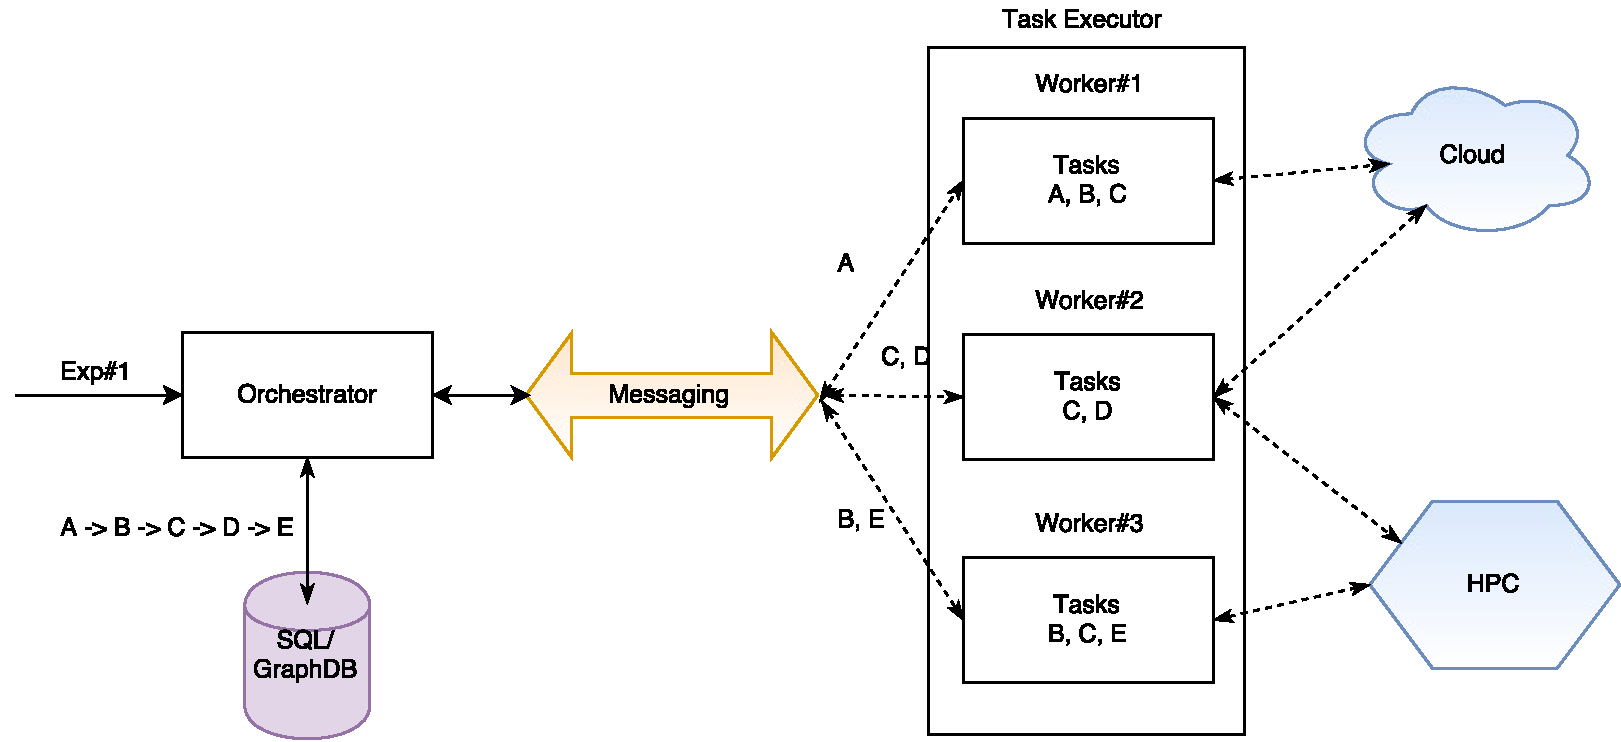
\includegraphics[height=2.2in, width=4.8 in]{figures/figure1.pdf}
\caption{The Orchestrator and Task Executor components communicate through a message bus that routes messages to workers following a publish-subscribe pattern. Workers 1-3 are capable of performing some subset of the tasks A, B, C, D, and E shown.}
\end{figure*}

For the orchestrator, there are two considerations that arise here:
\begin{itemize}
\item How does the Orchestrator know or decide which worker to pass the task execution to?
\item How do we upgrade a worker, say with a new task 'E' implementation, in such a manner that if something goes wrong with code for 'E', the entire worker node should not fail. In short, avoid regression testing the entire worker module.
\end{itemize}

To address the first consideration, we adopted a paradigm similar to Apache Aurora \cite{apacheAurora}.  Apache Aurora agents (workers) report available capabilities to the Aurora master (scheduler). In Aurora, the slave nodes constantly report back to the master how much processing power they have; accordingly, the master decides which slave to pass a new job request to. In our case, we can have the workers advertise to the orchestrator which tasks they are capable of executing and the orchestrator uses this information to make a decision as to which worker will execute a particular task.
Messaging systems such as those based on the AMQP specification can be used to offload orchestrator from scheduling part. We can delegate most of the responsibilities like service discovery, fault tolerance, and distributed coordination to a message infrastructure. This does mean however that the messaging system must be a highly available part of the system. Such coordination can also be accomplished with  frameworks like Apache Zookeeper \cite{hunt2010zookeeper} or Consul \cite{vargo2016consul}. We choose messaging approach implemented with RabbitMQ. 
To address the second consideration, every worker node can have independent task modules, such that if there is a problem with one task, it can be repaired without impacting other existing task implementations. Adding a new task implementation is simplified because each worker will report back to the orchestrator their capability to handle that new task. Likewise, new workers with new capabilities can be added to the system.  

Having a custom orchestrator also provides us benefits such as
\begin{itemize}
\item Handling failure conditions - for example, if a task execution on one worker fails, then the orchestrator can retry it on a different worker.
\item Prioritizing experiments - the orchestrator can send higher priority experiments to the workers that comprise the Task Executor before normal priority jobs.  
\item Delaying scheduling - the orchestrator can delay sending work to the Task Executor until a later time.   This could be used, for example, to avoid downtimes on remote execution resources. 
\end{itemize}

The Orchestrator is considered to be a highly available service and tracks the state of the tasks that it gives to the Task Executor.  The Orchestrator may be implemented following a leader election scheme to handle failures.  Because it uses externally stored DAGs to represent different task execution patterns, the Orchestrator has runtime mutability: we do not need to change the orchestrator code if we add a new task execution pattern. 

\section{SCALING AND UPGRADING}

Our system is consists of loosely-coupled microservices. Each microservice performs closely related functionalities and gives away work to others. As this is a microservice inspired architecture, it inherently supports scalability. Multiple instances of each microservice can be employed for load balancing. With this architecture, availability of the component can be realized by scaling microservices horizontally. The messaging infrastructure is a critical component and represents a single point of failure. We thus identify reliable communication infrastructure as a key attribute of any fabric, or substrate, system that would run the Orchestrator and Task Executor. We use RabbitMQ in our implementation. 

Our proposed design supports incremental upgrades; if a new task execution capability is added to a worker, other workers will continue to process task execution requests while the upgrade is in progress. Once the upgrade completes, this worker will now be able to accept and process requests for the new task type. Newly added capabilities are completely independent of existing ones, so the system does not require tedious regression testing. Also, these new capabilities can be incrementally replicated across multiple workers. As capabilities are added, Task Execution Patterns will be altered accordingly.  In other words, the system remains agnostic to any new implementations.

\section{IMPLEMENTATION AND EVALUATION}

\subsection{Implementation}
There is an obvious correlation between microservice communication and its impact on how the microservice performs the work assigned under specific circumstances. The design goal is to make sure we have maximum independence between microservices, and to fully investigate the workflow pattern in which these microservices will operate so we can find the right balance between availability and consistency.
The design is influenced by but not limited to specific task execution patterns followed in scientific applications.   We consider next a common pattern. 

\begin{figure*}
\centering
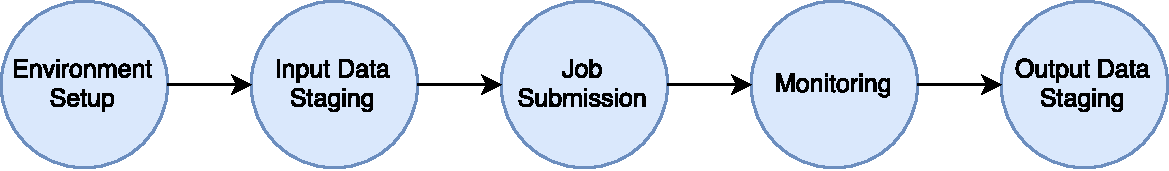
\includegraphics[height=0.8in, width=4.8 in]{figures/figure2.pdf}
\caption{List of tasks in a typical scientific application running on an HPC resource.}
\end{figure*}

Figure 2 illustrates a very basic pipeline for executing a task on an HPC resource, which is an exemplary use case for many science gateways.  More complicated execution graphs can be built up from this basic sequence. The steps are as follows:
\begin{itemize}
\item environment setup - creating directories and load modules for a job
\item staging input file - stage user input files on remote cluster
\item job execution - execute job execution commands
\item job status monitoring - monitor status of a job until it finishes
\item output data staging - after successful execution of a job transfer outputs files back in local environment.
\end{itemize}
Each of these is accounted as an independent task in our design. For each individual experiment, these tasks are bundled into a Task Execution Pattern. An experiment refers to a user request to run an application on a remote machine. Each component of our design is explained below with reference to example task definitions listed above.

\subsection{Orchestrator}
The orchestrator receives an experiment request, which indicates type of application to run on the remote machine, along with other parameters such as:
\begin{itemize}
\item The details of the remote resources; e.g., HPC cluster or cloud.
\item Remote resource identity.
\item The inputs to the application - could be files or data in terms of string, number
\item The details of the local storage; e.g. local machine where inputs are stored
\item Wall time, execution time, CPU count, execution time etc
\item The priority of the experiment - by default an experiment has NORMAL priority.
\item The scheduling time - by default the application will be scheduled to run immediately.
\end{itemize}
These parameters are coined as a TaskContext. The orchestrator retrieves appropriate Task Execution Pattern definition for an application from a graph store, such as a graph database, and constructs TaskContext for each task. The graph store maintains different execution patterns for different type of experiments. 
The orchestrator then publishes this TaskContext as a message via RabbitMQ broker to initiate execution of the task. The orchestrator tracks the state of the each task - per experiment - as it progresses through the execution pattern, and is responsible for handling errors and failures in task execution.

\subsection{Task Execution Workers}
We implement the abstract Task Execution component as a collection of workers. A worker can be equipped with one or more tasks. Based on installed capabilities, workers listen to message queues for incoming messages. When one worker takes up a task from a queue it is no longer available for other workers so that only one worker reacts to a task. If the worker fails send an acknowledgement, the Orchestrator queues the TaskContext again for other workers. Workers are responsible for executing instructions and transferring data to and from remote computing resources. Any new capability eventually can be replicated on multiple workers. 

\begin{figure}
\centering
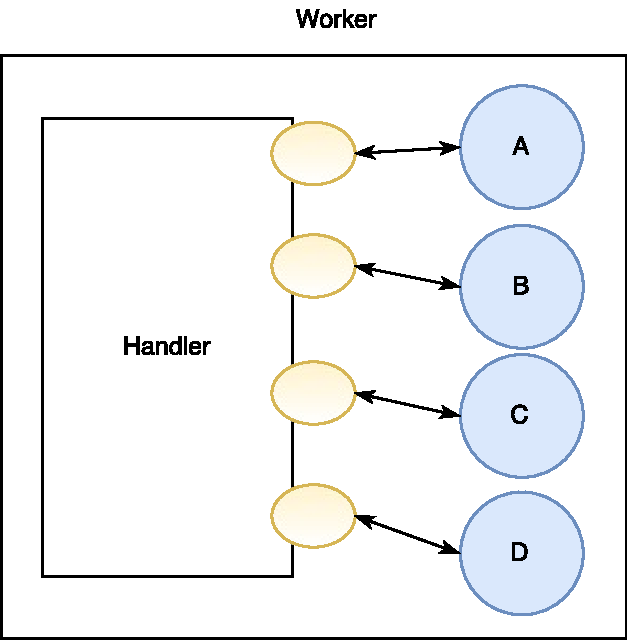
\includegraphics[height=1.8in, width=1.8 in]{figures/figure3.pdf}
\caption{Internal components of a Task Executor worker.}
\end{figure}

The worker depicted in Figure 3 has four task, A, B, C, and D. When the worker is started, it creates subscriber for each task, so in this case four subscribers are listening to queues corresponding to respective tasks. When subscriber receives a message, it invokes associated task implementation by passing the received TaskContext. When task execution is completed, based on execution status, a Response is created and sent back to orchestrator using a separates RabbitMQ queue.    
We implement a work-queue pattern within our messaging system, with workers configured to serve one or more tasks. Based on configuration, corresponding message queue subscribers are employed to listen to incoming messages. These subscribers simply invoke respective task implementations. The purpose of having a separate handler is to decouple tasks from how messages are communicated to workers, which makes these tasks independent modules for other frameworks. As shown in Figure 3, when a worker is started with four tasks, the handler simply creates corresponding listeners which in turn invoke respective implementations. To support new task, a worker needs to start a new subscriber in the handler associated with the task. 
Each task has a generic type and a more concrete implementation. Consider for example a Job Submission task, which can have different flavours with specific implementations for various remote clusters such as SLURM, Torque, HTCondor, and others. Even though this different flavors come under a same hood each maintains its own ecosystem. Each task type has single point of entry and from there control is passed to concrete implementation based on specific type mentioned in TaskContext. 

\subsection{Orchestrator - Worker interactions}

Each of the components described above is deployed as an independent microservice. Multiple instances of these components can be employed for fault tolerance and load balancing. RabbitMQ serves as message broker and sends data from one microservice to another.  Workers can be scaled horizontally to distribute load. Also, the tasks are embedded in such a way that each task can be scaled individually i.e. we can have multiple instances of particular task running on one machine. 

We base this implementation on \cite{sadooghi2014achieving}. In this model, the orchestrator is not logically aware of existing workers, or of their capabilities; therefore it does not make informed decisions about which worker will execute a given task.  To execute a task, the orchestrator publishes a TaskContext to the respective task message queue for any worker to process. The orchestrator receives a response from a worker after execution of the assigned task - success or failure/exception, and then it acts on it accordingly.  

\begin{figure*}
\centering
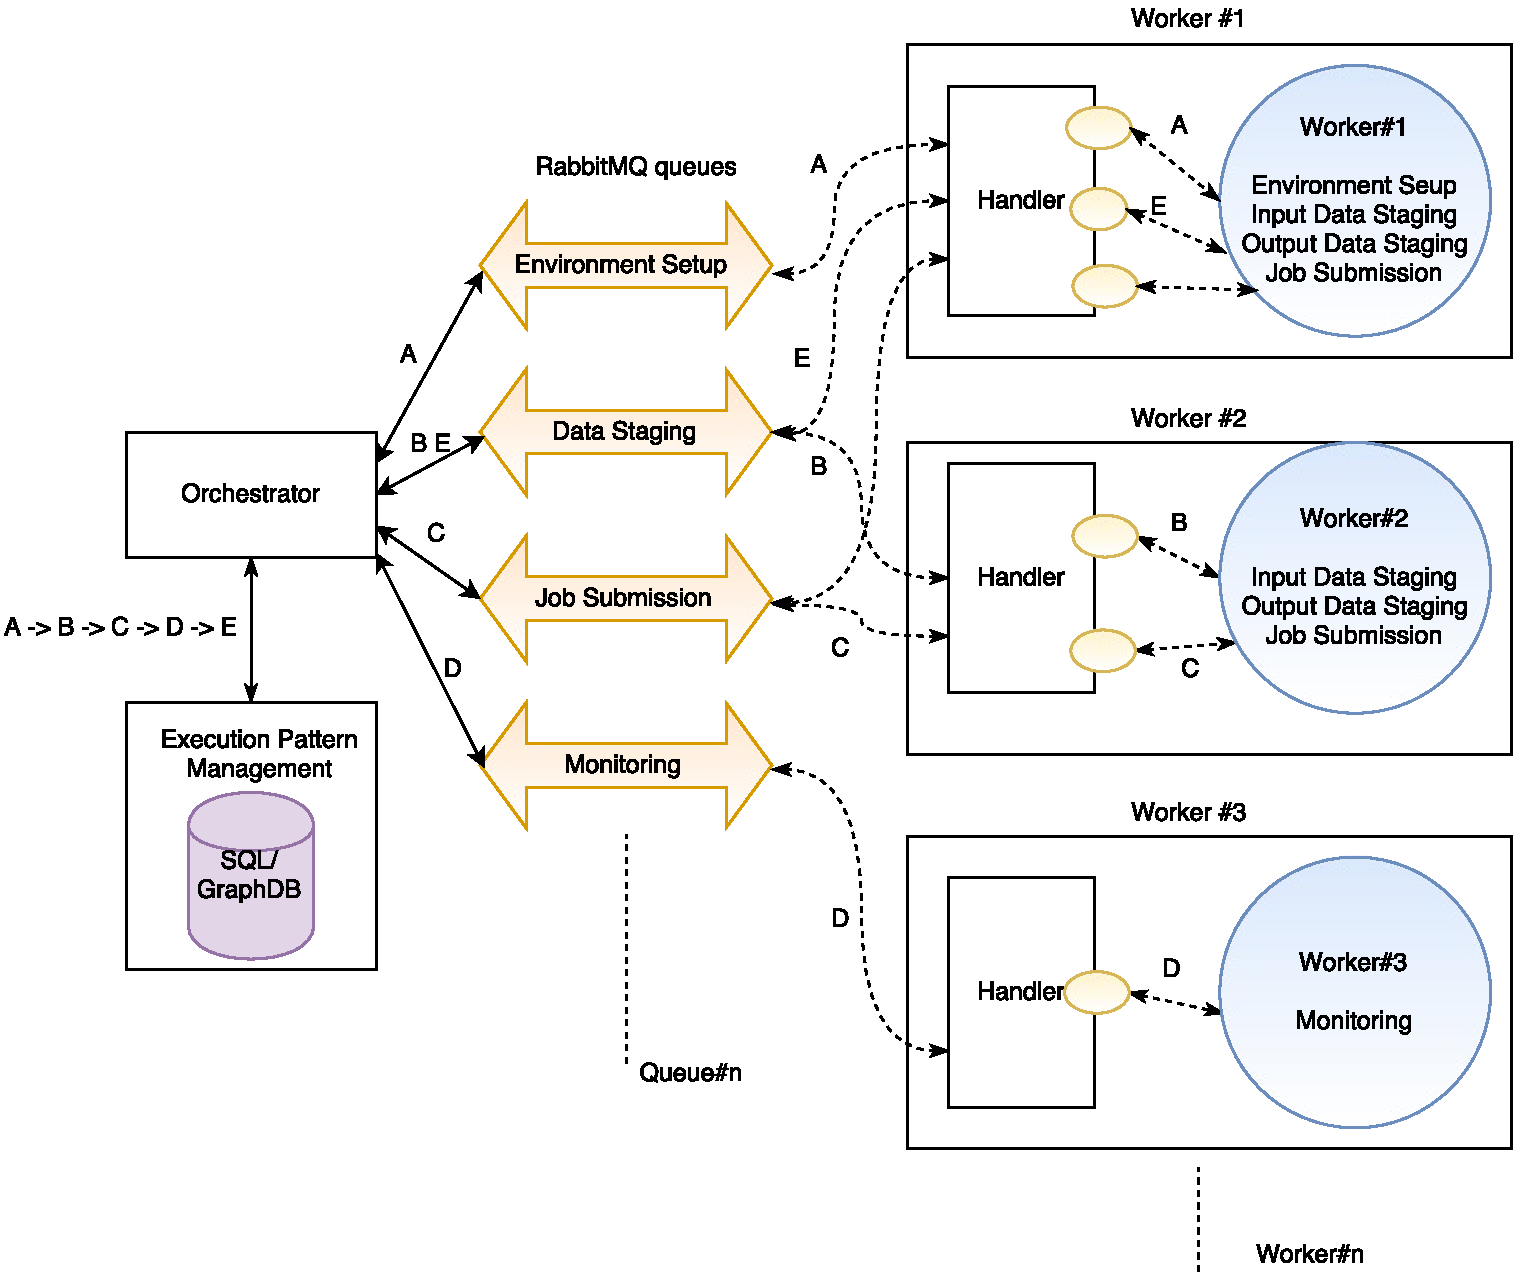
\includegraphics[height=3.8in, width=4.8 in]{figures/figure4.pdf}
\caption{Example message queues and workers for the task pipeline shown in in Figure 2. Solid arrows represent publish events and dashed arrow represent subscribe events.}
\end{figure*}

Let's address simple execution pattern A -> B -> C -> D -> E using Figure 4.  Workers have different capabilities and listen to different channels:
\begin{itemize}
\item Worker\#1 - Environment Setup, Data Staging (Input / Output), Job Submission
\item Worker\#2 - Data Staging (Input / Output), Job Submission
\item Worker\#3 - Monitoring
\end{itemize}

For simplicity, we annotate each task as follows:
\begin{itemize}
\item A  Environment Setup
\item B Input Data Staging
\item C Job Submission
\item D Monitoring
\item E Output Data Staging.
\end{itemize}

The steps are as follows. First, the orchestrator reads execution pattern from database based on experiment type, where it encounters task A and creates TaskContext for the same. Second, this task context is published to Environment Setup queue. Third, there can be one or multiple workers listening to this queue based on deployment; here Worker \#1 takes up and executes task A and responds back with result to orchestrator through queue. Finally, the Orchestrator reacts to the response message; in case of success, it marks task A as completed, fetches the subsequent task, creates a TaskContext and publishes it to Data Staging queue. If task is failed execution stops there and experiment is marked as failed.  This sequence is repeated until last task in execution pattern is executed successfully. The experiment is marked as completed if all succeed or failed otherwise.

\subsection{Using Fabric Services}

By nature, a framework needs to be as generic as possible with well-defined interfaces and hooks which can be extended with more concrete implementations based on specific requirements. The proposed framework is flexible enough to digest these requirements. Having validated the modularity aspect of the design, it is worth examining technologies that complement our framework and can best serve task execution.

The proposed design considers possibility of adapting to any new framework such as Spark, Flink, Mesos, Storm etc. The current framework uses RabbitMQ as a communication medium between orchestrator and workers. Here the framework specifically consists of part of an orchestrator which reacts to responses from worker and a handler in worker which accepts messages through RabbitMQ queues and calls respective task implementation.  

\subsection{Deployment}
We have discussed the validity, flexibility and robustness of the proposed framework. Now, it is important to consider deployment aspect for the same. The Orchestrator and the Task Executor's workers are microservices and hence can be deployed independently of other services in ecosystem. These components are good candidates for containerization, which open another dimension for deployment. A worker can be easily manipulated to start with one or more tasks which indeed serves as a microservice. So, these workers can be containers with multiple capabilities installed. 

These containers can be installed on Mesos cluster which would provide inherent fault tolerance. We have experimentally deployed the ecosystem described here on the Data Center Operation System (DC/OS), which is based on the Apache Mesos distributed system kernel. DC/OS is a distributed infrastructure as a service which abstracts out multiple machines as if they were a single computer. It facilitates resource management, process placement, inter-process communication and simplifies the installation and management of distributed services. This environment is best suitable for our framework to ensure load handling, resource utilization and fault tolerance.  


\section{RELATED WORK}

As discussed in sections 2 and 3 various facets of task execution challenges have been addressed over time in discussed extensively in distributed systems literature. Cyberinfrastructure projects have implemented these concepts in software systems to varying degree of successes. The larger vision of Apache Airavata [REF Design Considerations paper] is to leverage on existing systems to manage distributed task executions. In this paper, we share our experiences in building a particular implementation which will help us identify the challenges and possible generalizations. While it is not appropriate at this point to do a "apples to apples" comparison of this implementation with other platforms, we briefly discuss few projects who have tacked distributed task executions. 

As an example, HTCondor offers a robust workload management system for compute-intensive jobs. It provides a job queueing mechanism, scheduling, priority scheme, monitoring, and resource management. HTCondor employs a matchmaking algorithm to schedule jobs on particular nodes \cite{coleman2001implementation}. It uses ClassAd mechanism for matching resource requests (jobs) with nodes \cite{coleman2003distributed}. Whenever a job is submitted to Condor, it states both the requirements and the preferences, such as required memory, name of the program to run, user who submitted the job, and a rank for the node that will run the job. Also, nodes advertise their capacities in terms of RAM, CPU type and speed, current load with other static and dynamic properties.

Schedulers continuously read all the job ClassAds and all the node ClassAds and ensure that the requirement in both ClassAds are satisfied before scheduling any jobs on a node. HTCondor can be used to build a highly-scalable Grid-style computing environment.  It makes use of cutting edge Grid and cloud-based computing designs and protocols. HTCondor can be used to build Grid-style computing environments that cross administrative boundaries. 

One class of Airavata problems could potentially be addressed with HTCondor. As discussed in Section 2,  Science Gateways (hence Airavata) support multiple application patterns and also support Data Intensive Computing style workloads. We however see HTCondor could be integrated with Airavata, not as a framework, but as an adaptor to broker job submissions to High Throughput Computing workloads.   

As a next step with this effort, we would like to explore emerging large scale distributed systems like Apache Spark, Apache Storm and Apache Flink as viable alternative implementations to compare and potentially build upon to realize Airavata's goals. 


\section{CONCLUSIONS AND FUTURE WORK}
We have been able to come up with a flexible solution for distributed task execution. Considering its advantages, we are hoping to integrate this design in current Apache Airavata architecture. However, before Airavata code can absorb this framework it needs to go through rigorous testing cycles.

In its current capacity, the system supports pull mechanism between orchestrator and workers. Here, we are depending on messaging infrastructure (RabbitMQ) for delegating tasks to workers. This approach works well, but as we move ahead, systems might need to absorb surprising business demands.  Therefore, we prefer to retain control over task delegation rather than depending on third party technologies. The push mechanism would give better control over workers and task execution. One can think of using a matchmaking algorithm used by HTCondor where workers can advertise their capabilities in terms of task implementation, available memory, current load, CPU speed, etc.  In these situations the orchestrator can match task requirements with available workers and assign tasks accordingly. Also, the orchestrator can monitor node heartbeats to maintain workers? states and can spin up new instances as required. Again, one can think of gossip protocol to communicate state and resource information. Serf is a widely used gossip protocol which inherently supports scalability and fault tolerance.  

Also the system is open to adapt any new frameworks like Spark, Storm, Flink etc, which can handle resource management, fault tolerance, load balancing and communication between services. This would greatly offload Airavata from most of the orchestration and scheduling responsibilities.

Currently, we are using RabbitMQ as an underlying message infrastructure, considering it could be a single point of failure one can think of using a more robust, scalable and fault tolerant messaging infrastructure. Kafka is a very good contender, and we are planning to come up with better communication infrastructure which would satisfy the needs of scalability and fault-tolerance, yet give a very good control over message flow.

\bibliography{distributed-task-execution}

\end{document}
